\chapter*[Problema de Pesquisa]{Problema de Pesquisa}
\addcontentsline{toc}{chapter}{Problema de Pesquisa}

Como integrar leitura, tratamento e apresentação de dados de um Arduíno 
utilizando a linguagem R? Com base em minhas pesquisas identifiquei 
pouco conteúdo referente a leitura de dados de um Arduíno tendo o R como uma
interface. Das postagens que encontrei, a concepção da leitura dos dados 
necessitava de diversas 
interfaces\footnote{\url{https://magesblog.com/post/2012-10-02-connecting-real-world-to-r-with-arduino/}}
como outras linguagens e softwares, tirando a atratividade para pessoas que são 
novatas no assunto: conhecem o R porém pouco de Arduino, ou conhecem o 
Arduíno mas estão aprendendo R.

Por que utilizar o R? A linguagem de programação R, um dialeto da linguagem 
S, é amplamente utilizada em análise de dados e modelagem estatística. Possui 
código aberto sob licença GNU/GPL, resultando em milhares de pacotes criados 
pela comunidade, que atendem diversas áreas específicas. Seu uso era voltado 
a área de pesquisa mas acabou se difundido para a indústria. Atualmente 
diversas mídias especializadas mostram que a linguagem R cresce muito e de 
forma constante. Um exemplo é que, de acordo com o ranking de 2017 do 
IEEE\footnote{\url{https://spectrum.ieee.org/computing/software/the-2017-top-programming-languages}}
a linguagem R foi considerada a 6ª melhor linguagem de programação do ano conforme 
\autoref{r_ranking_I3E}, superando linguagens populares como PHP e 
JavaScript.

\begin{figure}[htb]
 \caption{\label{r_ranking_I3E} Ranking IEEE 2017}
 \begin{center}
  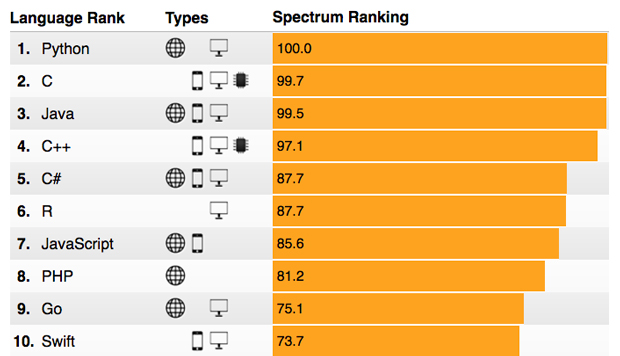
\includegraphics[scale = 0.4]{img/r_ranking_I3E.jpeg}
 \end{center}
\end{figure}

No tópico Ciência de Dados, R e Python são os mais utilizados. É difícil definir 
qual linguagem é melhor neste ponto, havendo diversos sites comparando-as.

Meu objetivo com a linguagem R é contribuir com a 
comunidade gerando conteúdo sobre Arduíno utilizando R, além de contribuir com 
abordagens de análise de dados para a comunidade do Arduino.

Por quê utilizar o Arduíno? 
\begin{citacao}[english]
  "When you start monitoring the environment,
  something happens: You start to understand the world around you in a new way." \cite{Gertz2012}
\end{citacao}

O baixo custo das plataformas de prototipagem, como Arduíno, a 
grande comunidade geradora de conhecimento e a filosofia \emph{open source}
possibilitam a qualquer pessoa, com pouco conhecimento em eletrônica, a
montar sistemas de medições de variáveis ambientais apenas seguindo exemplos 
disponíveis na internet. É possível encontrar: sistemas que medem umidade do 
solo, luminosidade de determinado local, turbidez, condutividade e ph da água, ruídos 
ambientais, e diversas outras variáveis, bastando ter apenas os sensores 
específicos. O Arduíno apresenta baixa complexidade, inclusive há escolas que o utilizam 
para ensino de eletrônica, robótica e programação no ensino médio.
 
Apesar de haver soluções simples\footnote{\url{https://magesblog.com/post/2015-02-17-reading-arduino-data-directly-into-r/}}
para o problema proposto, cabe a esta pesquisa adicionar mais elementos 
referente ao processo de análise de dados, além de fundamentação teórica nas 
etapas, tendo a linguagem de programação R como automatizadora do processo.